\documentclass[12pt,a4paper]{article}

% ---------- Page & fonts ----------
\usepackage[a4paper,margin=1.6cm,top=2cm,bottom=2cm]{geometry}
\usepackage{fontspec}
\setmainfont{Liberation Serif}
\setsansfont{Liberation Sans}
\usepackage{microtype}
\usepackage{setspace}
\setstretch{1.06}

% ---------- Color palette (matches the app's own brand colors) ----------
\usepackage[table]{xcolor}
\definecolor{eduBlue}{HTML}{2563EB}
\definecolor{eduBlueLight}{HTML}{DBEAFE}
\definecolor{eduGreen}{HTML}{059669}
\definecolor{eduGreenLight}{HTML}{D1FAE5}
\definecolor{eduYellow}{HTML}{F59E0B}
\definecolor{eduYellowLight}{HTML}{FEF3C7}
\definecolor{eduPurple}{HTML}{7C3AED}
\definecolor{eduPurpleLight}{HTML}{EDE9FE}
\definecolor{eduRed}{HTML}{E11D48}
\definecolor{eduRedLight}{HTML}{FFE4E6}
\definecolor{inkGray}{HTML}{1F2937}
\definecolor{softGray}{HTML}{6B7280}
\definecolor{pageBg}{HTML}{F7F9FC}

% ---------- Boxes, icons, layout tools ----------
\usepackage[most]{tcolorbox}
\usepackage{tikz}
\usetikzlibrary{arrows.meta}
\usepackage{graphicx}
\usepackage{enumitem}
\usepackage{array,tabularx,booktabs}
\usepackage{fancyhdr}
\usepackage{titlesec}
\usepackage{hyperref}

\hypersetup{
  colorlinks=true,
  linkcolor=eduBlue,
  urlcolor=eduBlue,
  citecolor=eduBlue,
  pdftitle={ShikshaSarthi Complete Guide},
  pdfauthor={ShikshaSarthi}
}

% ---------- Simple text-glyph "icons" (no external icon font needed) ----------
\newcommand{\iconAdmin}{\textbf{[SA]}}
\newcommand{\iconSchool}{\textbf{[SCH]}}
\newcommand{\iconTeacher}{\textbf{[T]}}
\newcommand{\iconStudent}{\textbf{[ST]}}
\newcommand{\iconArrow}{$\rightarrow$}

% ---------- Section styling ----------
\titleformat{\section}
  {\normalfont\Large\bfseries\color{eduBlue}}
  {\thesection}{0.5em}{}
\titleformat{\subsection}
  {\normalfont\large\bfseries\color{inkGray}}
  {\thesubsection}{0.5em}{}
\titlespacing*{\section}{0pt}{0.9em}{0.5em}
\titlespacing*{\subsection}{0pt}{0.8em}{0.35em}

% ---------- Header / footer ----------
\pagestyle{fancy}
\fancyhf{}
\renewcommand{\headrulewidth}{0.6pt}
\renewcommand{\footrulewidth}{0pt}
\fancyhead[L]{\small\color{eduBlue}\bfseries ShikshaSarthi}
\fancyhead[R]{\small\color{softGray} Complete Guide}
\fancyfoot[C]{\small\color{softGray}\thepage}

% ---------- Reusable colored role boxes ----------
\newtcolorbox{roleboxSA}{
  colback=eduPurpleLight, colframe=eduPurple, boxrule=1pt, arc=3mm,
  left=3mm, right=3mm, top=2mm, bottom=2mm, fonttitle=\bfseries,
  title={SUPER ADMIN}
}
\newtcolorbox{roleboxSCH}{
  colback=eduBlueLight, colframe=eduBlue, boxrule=1pt, arc=3mm,
  left=3mm, right=3mm, top=2mm, bottom=2mm, fonttitle=\bfseries,
  title={SCHOOL ADMIN}
}
\newtcolorbox{roleboxT}{
  colback=eduGreenLight, colframe=eduGreen, boxrule=1pt, arc=3mm,
  left=3mm, right=3mm, top=2mm, bottom=2mm, fonttitle=\bfseries,
  title={TEACHER}
}
\newtcolorbox{roleboxST}{
  colback=eduYellowLight, colframe=eduYellow, boxrule=1pt, arc=3mm,
  left=3mm, right=3mm, top=2mm, bottom=2mm, fonttitle=\bfseries,
  title={STUDENT}
}

% Q&A box
\newtcolorbox{qabox}[1]{
  colback=white, colframe=eduBlue, boxrule=1pt, arc=2.5mm,
  left=3mm, right=3mm, top=2mm, bottom=2mm,
  before skip=3mm, after skip=3mm,
  colbacktitle=eduBlue, coltitle=white, fonttitle=\bfseries,
  title={Q: #1}
}

% Tip / good-practice box (green)
\newtcolorbox{tipbox}{
  colback=eduGreenLight, colframe=eduGreen, boxrule=1pt, arc=2.5mm,
  left=3mm, right=3mm, top=1.7mm, bottom=1.7mm,
  before skip=2.5mm, after skip=2.5mm
}

% Warning box (red)
\newtcolorbox{warnbox}{
  colback=eduRedLight, colframe=eduRed, boxrule=1pt, arc=2.5mm,
  left=3mm, right=3mm, top=1.7mm, bottom=1.7mm,
  before skip=2.5mm, after skip=2.5mm
}

% Plain info box (blue)
\newtcolorbox{infobox}{
  colback=eduBlueLight, colframe=eduBlue, boxrule=1pt, arc=2.5mm,
  left=3mm, right=3mm, top=1.7mm, bottom=1.7mm,
  before skip=2.5mm, after skip=2.5mm
}

% ---------- Per-role step numbering (each restarts at 1) ----------
\newcounter{sasteps}
\newcounter{schsteps}
\newcounter{tsteps}
\newcounter{ststeps}

\newcommand{\sastep}[1]{\stepcounter{sasteps}\par\noindent{\bfseries\color{eduPurple}\thesasteps.} #1\par}
\newcommand{\schstep}[1]{\stepcounter{schsteps}\par\noindent{\bfseries\color{eduBlue}\theschsteps.} #1\par}
\newcommand{\tstep}[1]{\stepcounter{tsteps}\par\noindent{\bfseries\color{eduGreen}\thetsteps.} #1\par}
\newcommand{\ststep}[1]{\stepcounter{ststeps}\par\noindent{\bfseries\color{eduYellow!80!black}\theststeps.} #1\par}

\setlength{\parindent}{0pt}
\setlength{\parskip}{4pt}

\begin{document}
\pagecolor{pageBg}

% ============================================================ COVER PAGE
\begin{titlepage}
\pagecolor{white}
\newgeometry{margin=0cm}
\begin{tikzpicture}[remember picture, overlay]
  \fill[eduBlue] (current page.north west) rectangle ([yshift=-7.6cm]current page.north east);
  \fill[eduPurple, opacity=0.55] (current page.north west) rectangle ([yshift=-7.6cm, xshift=8cm]current page.north east);
\end{tikzpicture}

\vspace*{2.1cm}
\hspace{1.6cm}
\begin{minipage}{15cm}
{\color{white}\fontsize{44}{48}\selectfont\bfseries ShikshaSarthi}\\[0.3cm]
{\color{white}\Large Complete Guide for Everyone}\\[0.15cm]
{\color{white!85!black}\large Super Admin \(\cdot\) School Admin \(\cdot\) Teacher \(\cdot\) Student}
\end{minipage}

\vspace{2.3cm}
\hspace{1.6cm}
\begin{minipage}{14.5cm}
\begin{tcolorbox}[colback=white, colframe=eduBlue, boxrule=1.2pt, arc=3mm,
  left=5mm, right=5mm, top=3mm, bottom=3mm]
{\large\bfseries A short, simple manual} that explains what ShikshaSarthi does,
who uses it, how accounts connect to each other, and how the app stays updated
and synced --- even with unreliable internet.
\end{tcolorbox}
\end{minipage}

\vspace{1.4cm}
\hspace{1.6cm}
\begin{minipage}{14.5cm}
\renewcommand{\arraystretch}{1.5}
\begin{tabularx}{\linewidth}{@{}l X@{}}
\textbf{\textcolor{eduBlue}{Who is this for?}} & Super admins, school admins, teachers, and students \\
\textbf{\textcolor{eduGreen}{Works offline?}} & Yes --- designed for schools with patchy internet \\
\textbf{\textcolor{eduPurple}{Language}} & English and Hindi \\
\end{tabularx}
\end{minipage}

\vfill
\begin{center}
{\color{softGray}\small ShikshaSarthi --- Learning made simple, offline-first, for every school.}
\end{center}
\vspace{1cm}
\end{titlepage}
\restoregeometry
\pagecolor{pageBg}

% ============================================================ SECTION: INTRODUCTION
\section*{Introduction}
This application allows teachers to create, manage, and conduct quizzes offline on
computers. It is simple, fast, and does not require internet for normal usage. It
is best for schools with limited connectivity.

\section*{Installation Steps}
Follow these steps carefully:
\begin{enumerate}[leftmargin=*]
  \item Install the Quiz Application using the provided \texttt{.exe} setup file.
  \item Open the application after installation.
  \item No need to install anything else --- everything is already included.
\end{enumerate}

\textbf{Please read carefully:}
\begin{itemize}[leftmargin=*]
  \item No internet is required for basic usage.
  \item Internet is required only for the Sync feature.
  \item Data is stored locally in the system.
  \item For multi-system use, all devices must be on the same WiFi/LAN.
  \item Keep the main system ON when other systems are connected.
\end{itemize}

\textbf{For best performance:}
\begin{itemize}[leftmargin=*]
  \item Use one system as the server (teacher PC).
  \item Your Quiz Application is now fully ready to use. Connect all student systems using the IPv4 link.
  \item This ensures smooth quiz conduction without issues.
\end{itemize}

% ============================================================ SECTION: WHAT IS SHIKSHASARTHI
\section*{What is ShikshaSarthi?}
ShikshaSarthi is a school learning platform that works even when the internet does not.
Each school runs the app on its own local computer, so students and teachers can keep
teaching, practising, and testing all day --- with or without a working internet connection.

\begin{center}
\renewcommand{\arraystretch}{1.35}
\begin{tabularx}{\linewidth}{@{}>{\centering\arraybackslash}p{2.4cm} X@{}}
\rowcolor{eduPurpleLight}
\textbf{\textcolor{eduPurple}{\large SUPER\newline ADMIN}} & \textbf{Super Admin} --- runs the whole platform. Creates new schools and their first login. \\[4pt]
\rowcolor{eduBlueLight}
\textbf{\textcolor{eduBlue}{\large SCHOOL\newline ADMIN}} & \textbf{School Admin} --- runs one school. Adds teachers and students. \\[4pt]
\rowcolor{eduGreenLight}
\textbf{\textcolor{eduGreen}{\large TEACHER}} & \textbf{Teacher} --- runs classes. Creates classes, adds students, makes quizzes, checks results. \\[4pt]
\rowcolor{eduYellowLight}
\textbf{\textcolor{eduYellow!80!black}{\large STUDENT}} & \textbf{Student} --- learns and practises. Takes quizzes, adaptive tests, and multimedia activities. \\
\end{tabularx}
\end{center}

\begin{qabox}{Why do four different roles exist?}
Because a real school has four different jobs to do: one person runs the platform for
many schools (Super Admin), one person runs a single school (School Admin), many
people run classrooms (Teachers), and many people are learning (Students). Each
role only sees the tools it needs.
\end{qabox}

% ============================================================ SECTION: ARCHITECTURE
\section*{How everything connects}
Think of it as \textbf{one school computer + one small cloud helper} --- not one giant
central server that everyone depends on.

\begin{center}
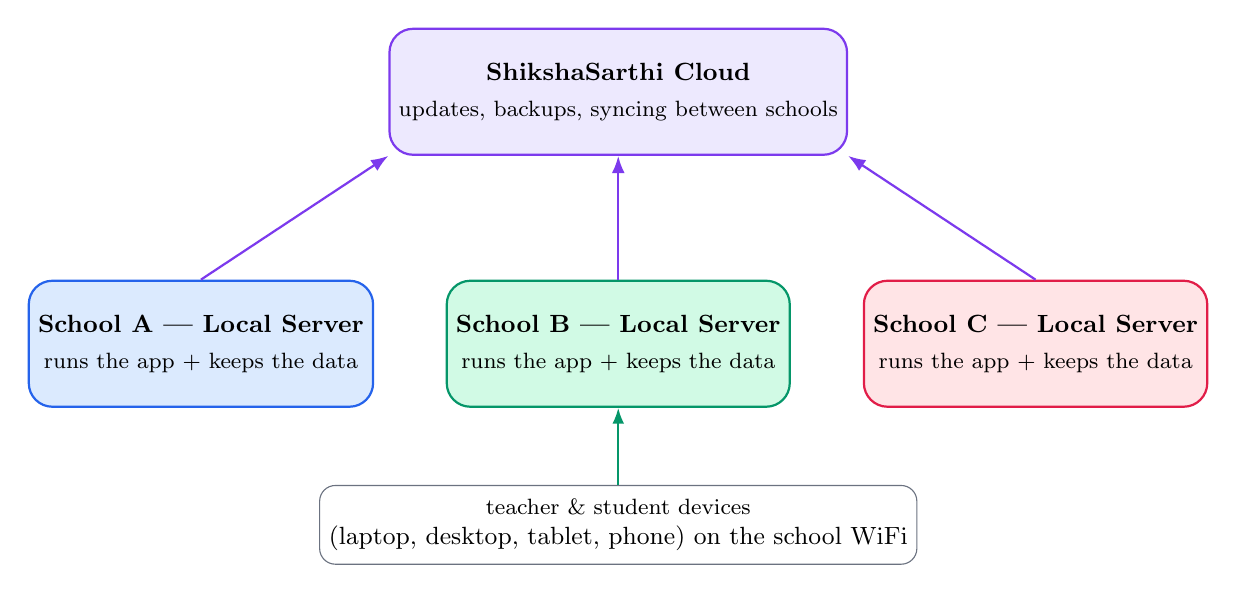
\begin{tikzpicture}[scale=1, every node/.style={font=\small}]
  % Cloud
  \node[draw=eduPurple, thick, fill=eduPurpleLight, rounded corners=3mm,
        minimum width=4.8cm, minimum height=1.6cm, align=center]
        (cloud) at (0,3.2) {\textbf{ShikshaSarthi Cloud}\\[2pt]\footnotesize updates, backups, syncing between schools};

  % Schools
  \node[draw=eduBlue, thick, fill=eduBlueLight, rounded corners=3mm,
        minimum width=4.3cm, minimum height=1.6cm, align=center]
        (school1) at (-5.3,0) {\textbf{School A --- Local Server}\\[2pt]\footnotesize runs the app + keeps the data};
  \node[draw=eduGreen, thick, fill=eduGreenLight, rounded corners=3mm,
        minimum width=4.3cm, minimum height=1.6cm, align=center]
        (school2) at (0,0) {\textbf{School B --- Local Server}\\[2pt]\footnotesize runs the app + keeps the data};
  \node[draw=eduRed, thick, fill=eduRedLight, rounded corners=3mm,
        minimum width=4.3cm, minimum height=1.6cm, align=center]
        (school3) at (5.3,0) {\textbf{School C --- Local Server}\\[2pt]\footnotesize runs the app + keeps the data};

  \draw[-{Latex[length=2.2mm]}, thick, eduPurple] (school1.north) -- (cloud.south west);
  \draw[-{Latex[length=2.2mm]}, thick, eduPurple] (school2.north) -- (cloud.south);
  \draw[-{Latex[length=2.2mm]}, thick, eduPurple] (school3.north) -- (cloud.south east);

  % Devices below school B as an example
  \node[draw=softGray, fill=white, rounded corners=2mm, minimum width=4.6cm, minimum height=1cm, align=center] (devices) at (0,-2.3) {\footnotesize teacher \& student devices\\ (laptop, desktop, tablet, phone) on the school WiFi};
  \draw[-{Latex[length=2mm]}, thick, eduGreen] (devices.north) -- (school2.south);
\end{tikzpicture}
\end{center}

\begin{infobox}
\textbf{The local school server is the ``main'' computer for that school.} It runs the
app and stores that school's data. Every teacher and student device (laptop, desktop,
tablet, phone) simply opens a web browser and connects to it over the school's own
WiFi or network --- like visiting a website, but the website lives inside the school.
\end{infobox}

\begin{infobox}
\textbf{The cloud is a helper, not a controller.} It does three things: (1) hands out
new app versions, (2) keeps a safety backup, and (3) quietly merges data between
schools when they choose to sync. Schools never talk to each other directly --- only
through the cloud, and the school keeps working perfectly even if the cloud is
unreachable.
\end{infobox}

\begin{qabox}{What happens if the internet goes down?}
Nothing breaks. The school's local server keeps running class, quizzes, and grading
normally. Only the cloud sync and update-check pause until the internet returns ---
they simply catch up automatically later.
\end{qabox}

\subsection*{How syncing works}
\begin{tipbox}
\textbf{Syncing means:} the school's local server quietly sends its new records
(new students, quiz results, classes) to the cloud, and pulls down anything new
from the cloud (like a shared question bank update). This happens automatically
in the background, and a Super Admin can also trigger it manually with one click.
\end{tipbox}

\subsection*{How updates work}
\begin{tipbox}
\textbf{Updates are safe by design.} The app checks the cloud for a newer version.
A Super Admin reviews it and chooses to install. Every update file is verified
before anything is installed, so a broken or incomplete download is automatically
rejected instead of damaging the school's data.
\end{tipbox}

\begin{warnbox}
\textbf{Updates never happen silently.} A Super Admin must always approve an
install. Student data, quiz history, and photos are never touched by an update ---
only the app program files change.
\end{warnbox}

\newpage
% ============================================================ SUPER ADMIN SECTION
\begin{roleboxSA}
The Super Admin manages the entire ShikshaSarthi platform --- every school on it.
\end{roleboxSA}

\section*{\textcolor{eduPurple}{1. Super Admin Guide}}

\subsection*{What can a Super Admin do?}
\begin{itemize}[leftmargin=1.3cm, itemsep=2pt]
  \item[\textcolor{eduPurple}{\textbullet}] Create a brand-new school, along with its first School Admin login.
  \item[\textcolor{eduPurple}{\textbullet}] Create or remove any account directly, in any school, if ever needed.
  \item[\textcolor{eduPurple}{\textbullet}] View statistics across every school on the platform.
  \item[\textcolor{eduPurple}{\textbullet}] Trigger cloud sync manually and check its status.
  \item[\textcolor{eduPurple}{\textbullet}] Check for, download, and install app updates.
\end{itemize}

\subsection*{Setting up a new school}
\setcounter{sasteps}{0}
\sastep{Open the Super Admin dashboard and choose \emph{Register School}.}
\sastep{Fill in the school's ID, name, location, and the details for its first School
  Admin: name, username, password, and phone number.}
\sastep{Submit. This creates the school \emph{and} its School Admin login in one step.}
\sastep{Share the School Admin's username and password with that school through a
  secure, trusted channel.}

\begin{warnbox}
Each school has exactly \textbf{one} School Admin account. Choose the person
carefully --- they will add every teacher and student for that school.
\end{warnbox}

\subsection*{Keeping the platform healthy}
\setcounter{sasteps}{0}
\sastep{Check \emph{Sync Status} regularly and press \emph{Sync Now} if a school reports
  a problem.}
\sastep{Check \emph{Check for Updates}; when a new version is ready, review the release
  notes before installing.}
\sastep{Use the platform-wide statistics to see which schools are active and which
  need support.}

\begin{qabox}{What if a School Admin forgets their password?}
The Super Admin can reset any School Admin's or Teacher's password directly.
Students use the school's approved recovery process, which a School Admin manages.
\end{qabox}

\newpage
% ============================================================ SCHOOL ADMIN SECTION
\begin{roleboxSCH}
The School Admin manages one school: its teachers, its students, and day-to-day
account issues.
\end{roleboxSCH}

\section*{\textcolor{eduBlue}{2. School Admin Guide}}

\subsection*{What can a School Admin do?}
\begin{itemize}[leftmargin=1.3cm, itemsep=2pt]
  \item[\textcolor{eduBlue}{\textbullet}] Add and remove Teacher accounts for this school.
  \item[\textcolor{eduBlue}{\textbullet}] Add and remove Student accounts for this school.
  \item[\textcolor{eduBlue}{\textbullet}] View this school's own statistics and rosters.
  \item[\textcolor{eduBlue}{\textbullet}] Manage their own profile and photo.
\end{itemize}

\begin{infobox}
A School Admin only ever sees and manages \textbf{their own school}. They cannot
see or change another school's data.
\end{infobox}

\subsection*{Adding a Teacher}
\setcounter{schsteps}{0}
\schstep{Log in with the credentials the Super Admin provided.}
\schstep{Open \emph{Manage Teachers} \iconArrow\ \emph{Add Teacher}.}
\schstep{Enter the teacher's ID, name, and a starting password.}
\schstep{Save. Share the login with the teacher directly.}

\subsection*{Adding a Student}
\setcounter{schsteps}{0}
\schstep{Open \emph{Manage Students} \iconArrow\ \emph{Add Student}.}
\schstep{Enter the student's ID, name, starting password, and batch/class year.}
\schstep{Save. The student can now log in --- a teacher will add them to a class
  next.}

\begin{tipbox}
\textbf{Tip:} keep a simple offline list (paper or spreadsheet) of every Student ID
and Teacher ID you create, matched to the real person's name. This makes password
recovery and roster checks much faster later.
\end{tipbox}

\begin{qabox}{Can a teacher add students themselves?}
A teacher enrols \emph{existing} students into their classes, but the student
account itself is created by the School Admin first. Think of it as: School Admin
issues the ID card, Teacher invites them into class.
\end{qabox}

\newpage
% ============================================================ TEACHER SECTION
\begin{roleboxT}
The Teacher runs classes: creating them, adding students, sharing material,
building quizzes, and reviewing results.
\end{roleboxT}

\section*{\textcolor{eduGreen}{3. Teacher Guide}}

\subsection*{What can a Teacher do?}
\begin{itemize}[leftmargin=1.3cm, itemsep=2pt]
  \item[\textcolor{eduGreen}{\textbullet}] Create classes and enrol students into them.
  \item[\textcolor{eduGreen}{\textbullet}] Post announcements and share documents with a class.
  \item[\textcolor{eduGreen}{\textbullet}] Build a question bank and create quizzes (MCQ, audio, video, puzzle).
  \item[\textcolor{eduGreen}{\textbullet}] View quiz analytics and each student's progress.
\end{itemize}

\subsection*{Creating a class and adding students}
\setcounter{tsteps}{0}
\tstep{Open \emph{Manage Classes} and choose \emph{Create Class} (top-right).}
\tstep{Pick the class number and subject, and add a short description.}
\tstep{Open the new class and choose \emph{Manage Students}.}
\tstep{Enter each Student ID to enrol them. Students only see quizzes posted
  \emph{after} they join.}

\subsection*{Creating a quiz}
\setcounter{tsteps}{0}
\tstep{Open \emph{Create Quiz} and give it a memorable Quiz ID.}
\tstep{Set a time limit and how many MCQ / audio / video / puzzle questions to include.}
\tstep{Pick questions from the question bank, or add a custom question.}
\tstep{Set the start and end time, choose which class(es) can see it, then publish.}
\tstep{Share the Quiz ID and deadline with your class through an announcement.}

\begin{tipbox}
\textbf{Before publishing, double-check:} every question slot is filled, the answer
key is correct, and the time limit matches the number of questions.
\end{tipbox}

\subsection*{Reviewing results}
\setcounter{tsteps}{0}
\tstep{Open \emph{Quiz Analytics} and select the quiz.}
\tstep{Check the average score, and open \emph{Students} to see who needs help.}
\tstep{Use \emph{Manage Students} on a class to see one learner's full history:
  quizzes taken, adaptive tests, and their rating over time.}

\begin{qabox}{A student says they can't see a quiz. What do I check first?}
Confirm they are enrolled in the right class, and that the quiz was created
\emph{after} they joined (or is marked as a class-wide global quiz).
\end{qabox}

\newpage
% ============================================================ STUDENT SECTION
\begin{roleboxST}
The Student logs in, practises, takes tests, and reviews their own results.
\end{roleboxST}

\section*{\textcolor{eduYellow!75!black}{4. Student Guide}}

\subsection*{What can a Student do?}
\begin{itemize}[leftmargin=1.3cm, itemsep=2pt]
  \item[\textcolor{eduYellow!80!black}{\textbullet}] Practise questions by subject and topic.
  \item[\textcolor{eduYellow!80!black}{\textbullet}] Take an Adaptive Test that adjusts to each answer.
  \item[\textcolor{eduYellow!80!black}{\textbullet}] See class announcements, files, and quizzes in \emph{My Classes}.
  \item[\textcolor{eduYellow!80!black}{\textbullet}] Try audio, video, puzzle, and Mental Ability activities.
  \item[\textcolor{eduYellow!80!black}{\textbullet}] Review any past quiz result, any time.
\end{itemize}

\subsection*{A simple daily routine}
\setcounter{ststeps}{0}
\ststep{Log in and check \emph{My Classes} for new announcements or quizzes.}
\ststep{Choose one activity: Practice, Adaptive Test, or a class quiz.}
\ststep{Read every question carefully before answering; use hints sparingly.}
\ststep{Submit, then look at what you got wrong --- not just the score.}
\ststep{Log out, especially on a shared school computer.}

\subsection*{Taking an Adaptive Test}
\setcounter{ststeps}{0}
\ststep{Open \emph{Adaptive Test} from the dashboard.}
\ststep{Choose a mixed test or a single subject.}
\ststep{Choose how many questions: 10, 20, 30, 40, or no limit.}
\ststep{Answer each question; the next question adapts to how you are doing.}
\ststep{Submit when ready --- your rating updates automatically.}

\begin{tipbox}
\textbf{Remember:} the rating is a learning signal, not a grade to fear. A lower
score simply points to what to practise next.
\end{tipbox}

\begin{warnbox}
Never share your Student ID or password with anyone else, and never take a
quiz for another student --- unless it is clearly marked as a \emph{Group Quiz}.
\end{warnbox}

\begin{qabox}{Can I review a quiz after I've already submitted it?}
Yes. Open the quiz from your reports at any time to see each question, your
answer, and the correct answer --- there is no time limit on reviewing.
\end{qabox}

\vspace{0.4cm}
\begin{center}
\begin{tcolorbox}[colback=eduBlue, colframe=eduBlue, arc=3mm, width=0.92\linewidth,
  left=4mm, right=4mm, top=2.5mm, bottom=2.5mm]
\centering{\color{white}\large\bfseries Learn with purpose. Teach with evidence. Keep every learner moving forward.}
\end{tcolorbox}
\end{center}

\end{document}
